%%%%%%%%%%%%%%%%%%%%%%%%%%%%%%%%%%%
%This is the LaTeX ARTICLE template for RSC journals
%Copyright The Royal Society of Chemistry 2016
%%%%%%%%%%%%%%%%%%%%%%%%%%%%%%%%%%%

\documentclass[twoside,twocolumn,9pt]{article}
\usepackage{extsizes}
\usepackage[super,sort&compress,comma]{natbib} 
\usepackage[version=3]{mhchem}
\usepackage[left=1.5cm, right=1.5cm, top=1.785cm, bottom=2.0cm]{geometry}
\usepackage{balance}
\usepackage{mathptmx}
\usepackage{amssymb} %additional package needed to make maths work
\usepackage{sectsty}
\usepackage{graphicx} 
\usepackage{lastpage}
\usepackage[format=plain,justification=justified,singlelinecheck=false,font={stretch=1.125,small,sf},labelfont=bf,labelsep=space]{caption}
\usepackage{float}
\usepackage{fancyhdr}
\usepackage{fnpos}
\usepackage[english]{babel}
\addto{\captionsenglish}{%
  \renewcommand{\refname}{Notes and references}
}
\usepackage{array}
\usepackage{droidsans}
\usepackage{charter}
\usepackage[T1]{fontenc}
\usepackage[usenames,dvipsnames]{xcolor}
\usepackage{setspace}
\usepackage[compact]{titlesec}
\usepackage{hyperref}
\usepackage{booktabs}
\usepackage{makecell}
\definecolor{Pink}{RGB}{255, 0, 255}
%%%Please don't disable any packages in the preamble, as this may cause the template to display incorrectly.%%%


\usepackage{epstopdf}%This line makes .eps figures into .pdf - please comment out if not required.

\definecolor{cream}{RGB}{222,217,201}

%%%%%%%%% Preamble of the bibliography, can be commented or deleted 
\def\bibpreamble{For the reference section, the style file \texttt{rsc.bst} can be used to generate the correct reference style.\footnotemark[4]
\begin{enumerate}
\item{Citations should appear here in the format A. Name, B. Name and C. Name, \emph{Journal Title}, 2000, \textbf{35}, 3523;} 
\item{A. Name, B. Name and C. Name, \emph{Journal Title, 2000}, \textbf{35}, 3523.}
\end{enumerate}
... \\\\
We encourage the citation of primary research over review articles, where appropriate, in order to give credit to those who first reported a finding. \href{https://www.rsc.org/news-events/articles/2020/jun/rsc-signs-dora/}{Find out more about our commitments to the principles of San Francisco Declaration on Research Assessment (DORA).}}
%%%%%%%%% 

\begin{document}

\pagestyle{fancy}
\thispagestyle{plain}
\fancypagestyle{plain}{
%%%HEADER%%%
\renewcommand{\headrulewidth}{0pt}
}
%%%END OF HEADER%%%

%%%PAGE SETUP - Please do not change any commands within this section%%%
\makeFNbottom
\makeatletter
\renewcommand\LARGE{\@setfontsize\LARGE{15pt}{17}}
\renewcommand\Large{\@setfontsize\Large{12pt}{14}}
\renewcommand\large{\@setfontsize\large{10pt}{12}}
\renewcommand\footnotesize{\@setfontsize\footnotesize{7pt}{10}}
\makeatother

\renewcommand{\thefootnote}{\fnsymbol{footnote}}
\renewcommand\footnoterule{\vspace*{1pt}% 
\color{cream}\hrule width 3.5in height 0.4pt \color{black}\vspace*{5pt}} 
\setcounter{secnumdepth}{5}

\makeatletter 
\renewcommand\@biblabel[1]{#1}            
\renewcommand\@makefntext[1]% 
{\noindent\makebox[0pt][r]{\@thefnmark\,}#1}
\makeatother 
\renewcommand{\figurename}{\small{Fig.}~}
\sectionfont{\sffamily\Large}
\subsectionfont{\normalsize}
\subsubsectionfont{\bf}
\setstretch{1.125} %In particular, please do not alter this line.
\setlength{\skip\footins}{0.8cm}
\setlength{\footnotesep}{0.25cm}
\setlength{\jot}{10pt}
\titlespacing*{\section}{0pt}{4pt}{4pt}
\titlespacing*{\subsection}{0pt}{15pt}{1pt}
%%%END OF PAGE SETUP%%%

%%%FOOTER%%%
\fancyfoot{}
\fancyfoot[LO,RE]{\vspace{-7.1pt}
\includegraphics[height=9pt]{head_foot/LF}}
\fancyfoot[CO]{\vspace{-7.1pt}\hspace{13.2cm}
\includegraphics{head_foot/RF}}
\fancyfoot[CE]{\vspace{-7.2pt}\hspace{-14.2cm}
\includegraphics{head_foot/RF}}
\fancyfoot[RO]{\footnotesize{\sffamily{1--\pageref{LastPage} ~\textbar  \hspace{2pt}\thepage}}}
\fancyfoot[LE]{\footnotesize{\sffamily{\thepage~\textbar\hspace{3.45cm} 1--\pageref{LastPage}}}}
\fancyhead{}
\renewcommand{\headrulewidth}{0pt} 
\renewcommand{\footrulewidth}{0pt}
\setlength{\arrayrulewidth}{1pt}
\setlength{\columnsep}{6.5mm}
\setlength\bibsep{1pt}
%%%END OF FOOTER%%%

%%%FIGURE SETUP - please do not change any commands within this section%%%
\makeatletter 
\newlength{\figrulesep} 
\setlength{\figrulesep}{0.5\textfloatsep} 

\newcommand{\topfigrule}{\vspace*{-1pt}% 
\noindent{\color{cream}\rule[-\figrulesep]{\columnwidth}{1.5pt}} }

\newcommand{\botfigrule}{\vspace*{-2pt}% 
\noindent{\color{cream}\rule[\figrulesep]{\columnwidth}{1.5pt}} }

\newcommand{\dblfigrule}{\vspace*{-1pt}% 
\noindent{\color{cream}\rule[-\figrulesep]{\textwidth}{1.5pt}} }

\makeatother
%%%END OF FIGURE SETUP%%%

%%%TITLE, AUTHORS AND ABSTRACT%%%
\twocolumn[
  \begin{@twocolumnfalse}
{
\includegraphics[height=30pt]{head_foot/journal_name}\hfill\raisebox{0pt}[0pt][0pt]{
\includegraphics[height=55pt]{head_foot/RSC_LOGO_CMYK}}\\[1ex]

\includegraphics[width=18.5cm]{head_foot/header_bar}}\par
\vspace{1em}
\sffamily
\begin{tabular}{m{4.5cm} p{13.5cm} }


\includegraphics{head_foot/DOI} & \noindent\LARGE{\textbf{Can PFAS adsorbents be predictively identified through machine learning? A study of PFOA-targeted screening in metal–organic frameworks$^\dag$}} \\%Article title goes here instead of the text "This is the title"
\vspace{0.3cm} & \vspace{0.3cm} \\

 & \noindent\large{M.~Hasan Mansoor,$^{\ast}$\textit{$^{a}$} Sousa Javan Nikkah,\textit{$^{b\ddag}$} Mosab Bazargani,\textit{$^{a\ddag}$} and Soumya Mukherjee\textit{$^{b}$}} \\%Author names go here instead of "Full name", etc.

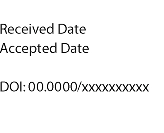
\includegraphics{head_foot/dates} & \noindent\normalsize{The freshwater and drinking-water PFAS problem; Why PFOA is used as a prototype contaminant; Why database-led predictive discovery is needed; Core workflow: labelled literature set + unlabelled CoRE-MOF/CSD discovery space + simulation-informed ML refinement; Key outcome: predictive identification of chemically plausible benchmark adsorbents; General significance for PFAS sorbent discovery. Any references in the abstract should be written out in full \textit{e.g.}\ [Surname \textit{et al., Journal Title}, 2000, \textbf{35}, 3523].} \\%The abstrast goes here instead of the text "The abstract should be..."

\end{tabular}

 \end{@twocolumnfalse} \vspace{0.6cm}

  ]
%%%END OF TITLE, AUTHORS AND ABSTRACT%%%

%%%FONT SETUP - please do not change any commands within this section
\renewcommand*\rmdefault{bch}\normalfont\upshape
\rmfamily

\vspace{-1cm}


%%%FOOTNOTES%%%

\footnotetext{\textit{$^{a}$~Address, Address, Town, Country. Fax: XX XXXX XXXX; Tel: XX XXXX XXXX; E-mail: xxxx@aaa.bbb.ccc}}
\footnotetext{\textit{$^{b}$~Address, Address, Town, Country. }}

%Please use \dag to cite the ESI in the main text of the article.
%If you article does not have ESI please remove the the \dag symbol from the title and the footnotetext below.
%\footnotetext{\dag~Supplementary Information available: [details of any supplementary information available should be included here]. See DOI: 00.0000/00000000.}
%additional addresses can be cited as above using the lower-case letters, c, d, e... If all authors are from the same address, no letter is required

\footnotetext{\dag~Additional footnotes to the title and authors can be included \textit{e.g.}\ `Present address:' or `These authors contributed equally to this work' as above using the symbols: \ddag, \textsection, and \P. Please place the appropriate symbol next to the author's name and include a \texttt{\textbackslash footnotetext} entry in the the correct place in the list.}


%%%END OF FOOTNOTES%%%

\section{Introduction}
\begin{enumerate}
	\item PFAS contamination as a freshwater and drinking-water challenge
	\item Why current sorbent discovery remains too slow and too empirical
	\item PFOA as a chemically and regulatorily meaningful prototype among PFAS
	\item Why metal--organic frameworks are attractive as tunable sorbents
	\item Why the Cambridge Structural Database and CoRE-MOF subsets create a discovery opportunity
	\item Why predictive design is still missing for PFAS-active metal--organic sorbents
	\item Study hypothesis and paper objective
\end{enumerate}

\textbf{Rough draft}: Per- and polyfluoroalkyl substances (PFAS) have become pervasive contaminants of freshwater and drinking-water supplies. Their widespread use in industrial processes and consumer products, coupled with the exceptional stability of their fluorinated carbon chains, has led to their persistence across aquatic environments. Continued exposure to several PFAS has been associated with adverse health outcomes, while increasingly stringent drinking-water limits require their removal at concentrations approaching the $ng L^{-1}$ regime. These demands present a formidable separation challenge: PFAS must be selectively scavenged from chemically complex aqueous matrices despite their low concentrations, diverse chain lengths and amphiphilic character.

Adsorption remains the most readily deployable technology for PFAS removal. Activated carbons are widely used, but their performance can be limited by slow uptake, competition from dissolved organic matter, poor affinity for shorter-chain PFAS and energy-intensive regeneration. These shortcomings have motivated the search for regenerable sorbents whose chemical environments can be tailored to recognise PFAS selectively. Metal–organic frameworks (MOFs) are particularly attractive in this regard because their pore dimensions, surface chemistry, hydrophobicity, charge distribution and metal–ligand composition can, in principle, be controlled independently. Recent studies have further shown that PFAS uptake cannot be rationalised by accessible surface area or pore volume alone. Rather, the interplay between confinement, hydrophobic association and electrostatic interactions appears to govern adsorption, highlighting the need for a multidimensional approach to sorbent design.

The chemical diversity that makes MOFs promising also makes their discovery experimentally intractable. The Cambridge Structural Database contains an extensive and continually expanding collection of experimentally reported metal–organic materials, while computation-ready subsets such as the CoRE-MOF databases provide thousands of structures suitable for systematic analysis. Only a small fraction (xx\%) of this structural space has been examined for PFAS adsorption, however, and an even smaller number has been evaluated under environmentally relevant conditions. Exhaustive synthesis and testing are therefore impractical, whereas high-level molecular simulations remain too computationally demanding to apply indiscriminately across the full database. Consequently, potentially exceptional adsorbents may remain hidden within a largely unexplored chemical space.

Machine learning offers a means of navigating this space, but its application to PFAS sorbent discovery is complicated by sparse and heterogeneous training data. Most reported studies describe materials that perform well, while rigorously defined inactive or poorly performing examples are scarce. Moreover, conventional geometric descriptors—including pore-limiting diameter, largest cavity diameter, accessible surface area, void fraction and framework density—cannot fully encode the chemical interactions responsible for PFAS binding. Predictive screening must therefore learn from limited labelled data while accounting for both framework geometry and chemical identity. Incorporating targeted molecular simulations into the learning cycle provides an additional route to overcome this limitation: candidates selected across the predicted performance range can be simulated, their interaction energies returned to the model, and the resulting expanded dataset used to refine subsequent predictions.

Here, we ask whether PFAS adsorbents can be prospectively identified through such an iterative, machine-learning-guided strategy. Perfluorooctanoic acid (PFOA) was selected as a prototypical target because it is a well-studied legacy C8 PFAS that combines a hydrophobic perfluoroalkyl chain with an anionic carboxylate headgroup, thereby capturing several of the competing interactions central to PFAS adsorption. We combine a curated set of MOFs with known or inferred PFOA adsorption behaviour with an unlabelled, computation-ready MOF search space. Structural descriptors calculated using Zeo++ are used to construct an initial predictive model, after which candidates spanning high-, intermediate- and low-ranking regions are subjected to molecular simulation. Iterative incorporation of the calculated PFOA–framework interaction energies enables the model to evolve from an initial sparse-label classifier towards a quantitative ranking framework.

Rather than replacing simulation or experiment, this approach uses machine learning to determine where these resource-intensive methods are most informative. In doing so, it provides both a shortlist of candidate PFOA adsorbents and a chemically interpretable assessment of the framework characteristics associated with strong binding. More broadly, the study establishes a transferable route for converting crystallographic databases into actionable discovery spaces for contaminant-selective sorbents.

\section{Literature Review / Data}

\begin{table*}[h]
	\begin{tabular}{lllccccccc}
		\hline
		\multicolumn{1}{c}{\textbf{\#}} &
		\multicolumn{1}{c}{\textbf{Name}} &
		\multicolumn{1}{c}{\textbf{Metal node}} &
		\textbf{\begin{tabular}[c]{@{}c@{}}Density \\ (g/cm\textasciicircum{}3)\end{tabular}} &
		\textbf{PLD(Å)} &
		\textbf{LCD (Å)} &
		\textbf{\begin{tabular}[c]{@{}c@{}}GSA \\ (m\textasciicircum{}2/g)\end{tabular}} &
		\textbf{\begin{tabular}[c]{@{}c@{}}Void \\ fraction\end{tabular}} &
		\textbf{\begin{tabular}[c]{@{}c@{}}Pore volume \\ (cm\textasciicircum{}3/g)\end{tabular}} &
		\textbf{\begin{tabular}[c]{@{}c@{}}Molecular weigth \\ of unit   cell(Å\textasciicircum{}2)\end{tabular}} \\ \hline
		1  & UiO-66          & Zr(IV)  & 1.23 & 3.82  & 8.70  & 2,921 & 0.59 & 0.48 & 6,640   \\
		2  & UiO-66-NH2      & Zr(IV)  & 2.02 & 1.28  & 7.33  & 2,383 & 0.42 & 0.21 & 10,960  \\
		3  & UiO-66-F4       & Zr(IV)  & 1.64 & 1.08  & 2.72  & 4,812 & 0.28 & 0.17 & 1,381   \\
		4  & UiO-67          & Zr(IV)  & 0.72 & 6.73  & 12.97 & 3,475 & 0.74 & 1.02 & 8,467   \\
		5  & UiO-67-F2       & Zr(IV)  & 0.86 & 6.64  & 12.83 & 3,059 & 0.72 & 0.84 & 10,194  \\
		6  & MOF-808         & Zr(IV)  & 1.28 & 10.09 & 15.64 & 2,178 & 0.63 & 0.49 & 33,373  \\
		7  & PCN-999         & Zr(IV)  & 0.59 & 18.48 & 19.44 & 3,430 & 0.79 & 1.34 & 19,228  \\
		8  & PCN-1002        & Zr(IV)  & 1.27 & 2.06  & 7.42  & 3,526 & 0.52 & 0.41 & 7,116   \\
		9  & DUT-67          & Zr(IV)  & 1.03 & 6.63  & 14.51 & 2,708 & 0.70 & 0.68 & 36,239  \\
		10 & NU-1000         & Zr(IV)  & 0.49 & 28.35 & 28.81 & 3,605 & 0.82 & 1.68 & 6,482   \\
		11 & MIL-53(Al)-as   & Al(III) & 1.00 & 5.95  & 6.52  & 3,991 & 0.59 & 0.59 & 13,254  \\
		12 & MIL-96(Al)      & Al(III) & 1.15 & 3.63  & 8.33  & 3,579 & 0.56 & 0.49 & 3,837   \\
		13 & MIL-100(Al)     & Al(III) & 0.68 & 8.50  & 27.81 & 3,593 & 0.74 & 1.09 & 150,561 \\
		14 & MIL-101(Cr)     & Cr(III) & 0.46 & 13.84 & 34.15 & 3,805 & 0.83 & 1.80 & 193,355 \\
		15 & MIL-101(Cr)-NH2 & Cr(III) & 1.87 & 1.16  & 2.33  & 4,245 & 0.36 & 0.19 & 4,081   \\
		16 & MIL-100 (Fe)    & Fe(III) & 0.76 & 8.85  & 27.76 & 3,271 & 0.74 & 0.97 & 180,331 \\
		17 & MIL-101 (Fe)    & Fe(III) & 0.46 & 13.84 & 34.15 & 3,805 & 0.83 & 1.80 & 193,355 \\
		18 & ZIF-7           & Zn(II)  & 1.44 & 3.13  & 4.35  & 3,930 & 0.44 & 0.31 & 2,076   \\
		19 & ZIF-8           & Zn(II)  & 0.92 & 3.58  & 11.98 & 4,996 & 0.64 & 0.69 & 2,707   \\
		20 & ZIF-L           & Zn(II)  & 1.50 & 1.07  & 2.36  & 5,397 & 0.35 & 0.23 & 7,344   \\
		21 & HKUST-1         & Cu(II)  & 0.95 & 5.21  & 11.12 & 3,707 & 0.69 & 0.72 & 10,446  \\
		22 & Mn-BTC          & Mn(II)  & 1.87 & 0.62  & 1.50  & 4,112 & 0.19 & 0.10 & 2,986   \\
		23 & Ce-BTC          & Ce(III) & 1.28 & 6.40  & 6.62  & 3,273 & 0.57 & 0.44 & 1,184  
	\end{tabular}
	\caption{Initial PFOA active list}
	\label{tab:Init-PFOA-active}
\end{table*}

\begin{itemize}
	\item \textbf{Defining the chemical question and the discovery workflow}
	\begin{enumerate}
		\item Literature-labelled active / inactive MOF space
		\item Database-mined unlabelled discovery space
		\item Relationship between Zeo++ descriptors, chemical descriptors, and adsorption behaviour
	\end{enumerate}
	
	\item \textbf{Building the descriptor space}
	\begin{enumerate}
		\item Geometric descriptors retained
		\item Chemical descriptors added
		\item Why topology was considered but not pursued in the final model
		\item Descriptor sparsity, collinearity, and dimensionality constraints
	\end{enumerate}
\end{itemize}
We start with 23 PFOA active MOFs known from literature  shown in Table~\ref{tab:Init-PFOA-active}. Each of these MOFs is know to be adsorption active for PFOA at various efficacy levels. However, because testing conditions across literature are unstandardised (such as MOF dosage, PFOA concentration, adsorption time, adsorption capacity, removal percentage etc.), we are unable to put a numerical score on each MOF's ability to remove PFOA. Consequently, we are only able to label these MOFs as `PFOA active'.

We capture seven numerical features for each MOF: density, pore limiting diameter (PLD), largest cavity diameter (LCD), geometric surface area (GSA), void fraction, pore volume and molecular weight per unit cell, also shown in Table~\ref{tab:Init-PFOA-active}. Large enough PLD and LCD are expected to allow PFOA adsorption, without being so large so as to not hold tightly to the PFOA molecule. These features are meant to capture the necessary (but not sufficient) condition for adsorption. GSA, void fraction and pore volume are expected to capture the capacity potential of adsorption, on the other hand. We also information available regarding the metal active node of the MOF and its density and molecular weight per unit cell for potential use in machine learning modelling.


\section{Methodology}\label{sec:method}

The ML--simulation based workflow starts from the 23 PFOA active MOFs in existing literature and is formed of three major steps:

\begin{enumerate}
	\item Baseline model (OCSVM) + binary simulation \textbf{1 iteration}
	\item SVM + energy simulatio \textbf{1 iteration}
	\item SVR + energy simulation \textbf{ iterations}
\end{enumerate}
We note novelty of architecture and application using existing machine learning modelling approaches.

\begin{figure}[!h]
	\centering
	\includegraphics[width=\linewidth]{figures/pipeline.png}
	\caption{Overall workflow.}
	\label{fig:ML-pipeline}
\end{figure}

\subsection{Baseline Single Class Labelling model (OCSVM)}\label{sec:method-1_OCSVM}

\begin{itemize}
	\item \textbf{Establishing the baseline predictive model}
	\begin{enumerate}
		\item Initial model trained on labelled data
		\item Positive-only or highly imbalanced learning rationale
		\item First-pass ranking of database candidates
	\end{enumerate}
\end{itemize}



The discovery of new PFAS-removing MOFs presents a challenge for conventional supervised learning approaches, as reliable negative examples are inherently difficult to define. While a subset of experimentally validated MOFs exhibiting strong PFAS adsorption performance can be identified from literature, the vast majority of available MOF structures lack corresponding adsorption measurements and cannot be confidently assigned as inactive. This creates a positive-unlabelled learning problem rather than a conventional binary classification task.

To address this challenge, we employ a One-Class Support Vector Machine (OC-SVM) approach, which is specifically designed to learn the characteristic feature space occupied by a single class. Unlike traditional support vector machines, which construct a maximum-margin hyperplane separating positive and negative samples, OC-SVM identifies a boundary enclosing the region of feature space associated with known positive examples. Although commonly applied for anomaly detection, including fraud identification and cybersecurity applications, the same principle can be adapted for materials discovery by defining successful PFAS-removing MOFs as the target class. The resulting model learns the structural and chemical characteristics associated with effective PFAS adsorption and enables the screening of unexplored MOFs within the CoRE MOF database prior to computationally expensive molecular simulations.

The descriptor vector of each experimentally reported PFAS-active MOF is represented as:
\begin{equation}
	\mathbf{x}_i\in \mathbb{R}^d, \qquad
	i= 1, \ldots, n,
	\label{eq:feature-vector}
\end{equation}

where $d$ represents the number of physicochemical descriptors used to define the MOF feature space. Since the literature-derived dataset contains only confirmed PFAS-adsorbing MOFs, with no reliable inactive examples, the initial classification problem was formulated as a one-class learning task.

The OC-SVM attempts to separate the mapped data from the origin by finding a hyperplane:
\begin{equation}
	\mathbf{w}^{T}\phi(\mathbf{x}) - \rho = 0\;,
	\label{eq:ocsvm-hyperplane}
\end{equation}

where: 
\begin{itemize}
	\item \( \phi(\mathbf{x}) \) is called the kernel. It allows for the features to be transformed to a higher dimension space thus allowing non-linear separating regions (instead of hyperplanes) to enclose (rather than separate) the data. We use the RBF kernel.
	\item \(\mathbf{w}\) are the coefficients on the now linear-in-kernel (not features) hyperplane. These can be thought of as the gradient or orienting parameters that can be manipulated to determine the separation of the hyperplane from the origin.
	\item \(\rho\) is the constant parameter that functions similarly in placing the hyperplane.
\end{itemize}

While the details of solving the optimisation problem that determine the best set of values for the orienting and constant parameters are not needed, we none the less briefly present the optimisation problem in order to motivate the hyper-parameters we must control. The OC-SVM is obtained by solving the following optimisation problem:

\begin{equation}
	\begin{aligned}
		\min_{\mathbf{w},\,\rho,\,\boldsymbol{\xi}}\quad
		& \frac{1}{2}\|\mathbf{w}\|^2
		+ \frac{1}{\nu n}\sum_{i=1}^{n}\xi_i
		- \rho \\
		\text{subject to}\quad
		& \mathbf{w}^{T}\phi(\mathbf{x}_i) \geq \rho - \xi_i,
		\qquad i=1,\ldots,n,\\
		& \xi_i \geq 0,
		\qquad i=1,\ldots,n.
	\end{aligned}
	\label{eq:ocsvm-primal}
\end{equation}

The minimisation across the two parameters \(w \text{ and } \rho\) fits the smallest boundary encompassing the data, however the introduction of an error term \(\epsilon\) allows fitting a tighter boundary, with the hyper-parameter \(\nu\) controlling the degree to which errors may be accepted. Figure~\ref{fig:OCSVM-train} shows the OC-SVM results based on hyper-parameter value of $\nu = 15\%$ (values between 5\% to 20\% showed similar results). The 23 PFOA active MOFs together define a region in the feature space that is visualised using a 2-PCA plot.
\begin{figure}[!h]
	\centering
	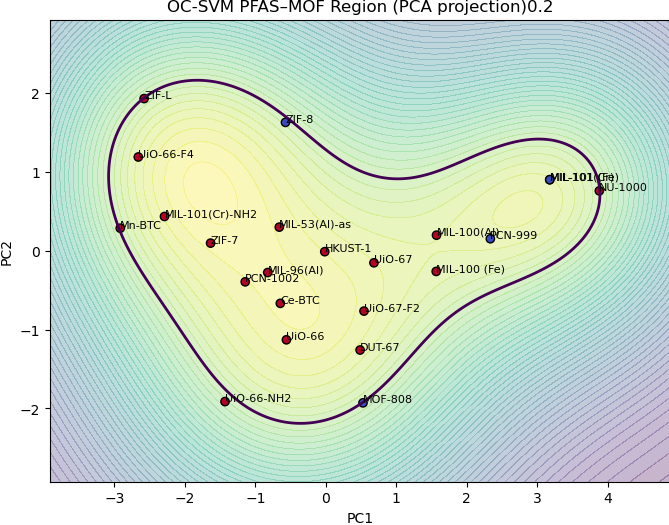
\includegraphics[width=\linewidth]{figures/OCSVM-Region-nu0.2.png}
	\caption{OCSVM results classifying the original 23 MOFs$^*$.}
	\label{fig:OCSVM-train}
\end{figure}
\footnotetext{\textit{$^{*}$~Reference Table~\ref{tab:Init-PFOA-active}}}


Once we have trained the OCSVM model, we are able to pass the features of any MOF and obtain a centrality score for the MOF. A high positive score indicates MOFs central to the region defined by the model, negative scores mean MOFs outside the region while a score of zero defines MOFs that lie on the frontier of the region.

Our next step becomes the validation of the OCSVM model via simulations, if the model is well defined highly positive scored MOFs will  return positive simulation while negatively scored ones will return negative simulation results. However, a point to note here is while simulations represent lower effort than physical experimentation, they none the less are time consuming.

Table~\ref{tab:OCSVM-result} represent a choice of the six highest scored MOFs from the coremofs database along with the three worst and two borderline MOFs, the six highest scored ones are predicted to be PFOA `Active', the three worst scored MOFs are predicted to be InActive while the borderline ones are assigned the `frontier' label. The last column represents the results of carrying out simulations on these MOFs. As can be seen `Active' predictions were all incorrect, mainly due PLD limitations, while the `Frontier' ones came back PFOA active. The model was able to correctly predict the simulation outcome for the `InActive' MOFs.


% \usepackage{booktabs} and \usepackage{makecell} needed
\begin{table*}[t]
	\centering
	\begin{tabular}{@{}lllllllllllll@{}}
		\toprule
		\textbf{Name} &
		\makecell{\textbf{OCSVM}\\\textbf{($\nu=0.15$)}} &
		\textbf{Density} &
		\textbf{PLD} &
		\textbf{LCD} &
		\textbf{GSA} &
		\makecell{\textbf{Void}\\\textbf{Fraction}} &
		\makecell{\textbf{Pore}\\\textbf{Volume}} &
		\makecell{\textbf{Molecular}\\\textbf{Weight}\\\textbf{(g/mol)}} &
		\makecell{\textbf{Stage 1}\\\textbf{OCSVM}\\\textbf{Prediction}} &
		\makecell{\textbf{Stage 1}\\\textbf{Simulation}\\\textbf{Result}} \\
		\midrule
		2008{[}Co{]}{[}sql{]}2{[}ASR{]}1  & 0.15         & 1.52 & 2.43  & 4.78  & 4,256 & 0.40 & 0.26 & 2,113 & Active   & NotGood  \\
		2018{[}Co{]}{[}flu{]}3{[}ASR{]}1  & 0.15         & 1.35 & 2.80  & 4.45  & 4,348 & 0.43 & 0.32 & 917   & Active   & NotGood  \\
		2022{[}Co{]}{[}gra{]}3{[}ASR{]}1  & 0.15         & 1.30 & 2.18  & 5.07  & 4,527 & 0.45 & 0.34 & 3,940 & Active   & NotGood  \\
		2015{[}Pr{]}{[}hcb{]}2{[}ASR{]}1  & 0.15         & 1.51 & 2.33  & 4.48  & 4,281 & 0.41 & 0.27 & 3,480 & Active   & NotGood  \\
		2023{[}Zn{]}{[}nan{]}3{[}ASR{]}13 & 0.15         & 1.51 & 2.31  & 4.47  & 4,462 & 0.41 & 0.27 & 2,909 & Active   & NotGood  \\
		2024{[}Cu{]}{[}pcu{]}3{[}ASR{]}2  & 0.15         & 1.42 & 2.33  & 4.03  & 4,418 & 0.41 & 0.29 & 5,405 & Active   & NotGood  \\
		2021{[}Eu{]}{[}fcu{]}3{[}ASR{]}2  & 0.00         & 0.79 & 7.21  & 14.75 & 3,040 & 0.76 & 0.96 & 2,505 & Frontier & Active   \\
		2022{[}Ni{]}{[}kgd{]}2{[}ASR{]}1  & -       0.00 & 0.83 & 3.23  & 9.75  & 5,091 & 0.61 & 0.73 & 946   & Frontier & Active   \\
		2015{[}Zr{]}{[}ftw{]}3{[}ASR{]}3  & -       0.65 & 0.29 & 10.50 & 25.26 & 4,625 & 0.87 & 3.00 & 4,241 & InActive & InActive \\
		2016{[}Mg{]}{[}stp{]}3{[}ASR{]}2  & -       0.67 & 0.28 & 26.59 & 28.06 & 4,802 & 0.88 & 3.08 & 2,538 & InActive & InActive \\
		2020{[}Fe{]}{[}hcb{]}2{[}ASR{]}2  & -       0.78 & 0.18 & 15.58 & 22.95 & 4,288 & 0.93 & 5.31 & 792   & InActive & InActive \\ \bottomrule
	\end{tabular}
	\caption{OCSVM prediction and simulation results for 11 selected COREMOFs}
	\label{tab:OCSVM-result}
\end{table*}

While these results are mixed, they give the necessary information to further refine the machine learning approach.

\subsection{Two-Class Classification Model (SVM)}\label{sec:method-2_SVM}

We are able to append the 11 CoRE MOFs from Table~\ref{tab:OCSVM-result} to the original 23 PFOA-active MOFs to obtain a dataset of 34 MOFs, comprising 25 positive and 9 negative samples. The labels of the additional MOFs were assigned from the molecular simulation results, with a positive label corresponding to a PFOA-active MOF and a negative label corresponding to a PFOA-inactive and frontier MOFs. This additional simulation-derived information transforms the initial positive-only learning problem into a conventional two-class classification problem.

A Support Vector Machine (SVM) was therefore employed to learn a decision boundary between the active and inactive MOFs. Given a set of labelled MOFs represented by descriptor vectors $\mathbf{x}_i$ and corresponding class labels $y_i \in \{-1,+1\}$, the separating hyperplane can be expressed as

\begin{equation}
	\mathbf{w}^{T}\phi(\mathbf{x}) + b = 0,
	\label{eq:svm-hyperplane}
\end{equation}

where $\mathbf{w}$ defines the orientation of the hyperplane, $b$ is the intercept, and $\phi(\mathbf{x})$ maps the input descriptor vector into the feature space. The optimal hyperplane is obtained by maximising the margin between the two classes. For a linearly separable dataset, this can be formulated as the minimisation problem

\begin{equation}
	\begin{aligned}
		\min_{\mathbf{w},\,b}\quad
		& \frac{1}{2}\|\mathbf{w}\|^2 \\
		\text{subject to}\quad
		& y_i\left(\mathbf{w}^{T}\phi(\mathbf{x}_i)+b\right) \geq 1,
		\qquad i=1,\ldots,n.
	\end{aligned}
	\label{eq:svm-hard}
\end{equation}

In practice, perfect separation of the active and inactive MOFs is not expected, particularly given the limited number of simulation-labelled samples. Slack variables $\xi_i$ were therefore introduced to permit individual observations to violate the margin, giving the soft-margin formulation

\begin{equation}
	\begin{aligned}
		\min_{\mathbf{w},\,b,\,\boldsymbol{\xi}}\quad
		& \frac{1}{2}\|\mathbf{w}\|^2
		+ C\sum_{i=1}^{n}\xi_i \\
		\text{subject to}\quad
		& y_i\left(\mathbf{w}^{T}\phi(\mathbf{x}_i)+b\right)
		\geq 1-\xi_i, \\
		& \xi_i \geq 0,
		\qquad i=1,\ldots,n,
	\end{aligned}
	\label{eq:svm-soft}
\end{equation}

where $C$ controls the trade-off between maximising the classification margin and penalising misclassified or margin-violating observations. A large value of $C$ places greater emphasis on correctly classifying the training data, whereas a smaller value permits greater tolerance of classification errors in favour of a wider margin.

For nonlinear separation of the MOF descriptor space, the mapping $\phi(\mathbf{x})$ can be avoided explicitly through the use of a kernel function,

\begin{equation}
	K(\mathbf{x}_i,\mathbf{x}_j)
	=
	\phi(\mathbf{x}_i)^{T}\phi(\mathbf{x}_j).
	\label{eq:svm-kernel}
\end{equation}

The resulting classification function can then be written in its kernelised form as

\begin{equation}
	f(\mathbf{x})
	=
	\sum_{i=1}^{n}\alpha_i y_i
	K(\mathbf{x}_i,\mathbf{x}) + b,
	\label{eq:svm-decision}
\end{equation}

where $\alpha_i$ are the coefficients obtained during optimisation and the observations with non-zero $\alpha_i$ constitute the support vectors. The predicted class is determined from the sign of the decision function,

\begin{equation}
	\hat{y} =
	\operatorname{sign}\left[f(\mathbf{x})\right].
	\label{eq:svm-classification}
\end{equation}

The SVM was subsequently trained using the combined set of literature-derived and simulation-labelled MOFs and applied to the remaining MOFs within the CoRE database. In contrast to the OC-SVM, which identified MOFs according to their similarity to the descriptor space of known PFOA-active materials, the two-class SVM was able to explicitly distinguish between descriptor characteristics associated with simulated PFOA-active and PFOA-inactive MOFs. The resulting classification was then used to identify a reduced set of candidate MOFs for the next round of molecular simulations.

\subsection{Support Vector Regression}
The simulation results, including the bond energies, obtained from these newly selected candidates were subsequently incorporated into the training dataset, providing additional labelled examples for refinement of the classification model and enabling progression to the next stage of the machine learning pipeline.


\section{Conclusions}
The conclusions section should come in this section at the end of the article, before the Author contributions statement and/or Conflicts of interest statement.

\section*{Author contributions}
We strongly encourage authors to include author contributions and recommend using \href{https://casrai.org/credit/}{CRediT} for standardised contribution descriptions. Please refer to our general \href{https://www.rsc.org/journals-books-databases/journal-authors-reviewers/author-responsibilities/}{author guidelines} for more information about authorship.

\section*{Conflicts of interest}
In accordance with our policy on \href{https://www.rsc.org/journals-books-databases/journal-authors-reviewers/author-responsibilities/#code-of-conduct}{Conflicts of interest} please ensure that a conflicts of interest statement is included in your manuscript here.  Please note that this statement is required for all submitted manuscripts.  If no conflicts exist, please state that ``There are no conflicts to declare''.

\section*{Data availability}


A data availability statement (DAS) is required to be submitted alongside all articles. Please read our \href{https://www.rsc.org/journals-books-databases/author-and-reviewer-hub/authors-information/prepare-and-format/data-sharing/#dataavailabilitystatements}{full guidance on data availability statements} for more details and examples of suitable statements you can use.

\section*{Acknowledgements}

The acknowledgements come at the end of an article after the conclusions and before the notes and references. 

%%%END OF MAIN TEXT%%%

%The \balance command can be used to balance the columns on the final page if desired. It should be placed anywhere within the first column of the last page.

\balance

%If notes are included in your references you can change the title from 'References' to 'Notes and references' using the following command:
%\renewcommand\refname{Notes and references}

%%%REFERENCES%%%
\bibliography{rsc} %You need to replace "rsc" on this line with the name of your .bib file
\bibliographystyle{rsc} %the RSC's .bst file
\end{document}
